\section{Tasks, Await und Async}

\begin{multicols*}{2}
\begin{itemize}
    \item Synchrone Operation
    \begin{itemize}
        \item Return aus der Methode nachdem die gesamte Logik durchlaufen wurde
        \item Blockieren den Aufrufer bis diese fertig gelaufen sind
    \end{itemize}
    \item Asynchrone Operation
    \begin{itemize}
        \item Ruft eine Methode auf ohne auf das Resultat zu warten
        \item Möglichkeit zur Benachrichtigung bei Fertigstellung (Callback) ODER Rückgabe eines Task Objektes auf welchem Status abgefragt werden kann
    \end{itemize}
\end{itemize}
\fat{Wichtig:}
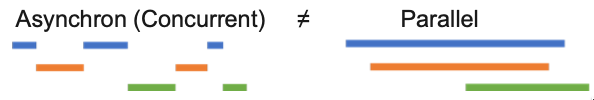
\includegraphics[width=\columnwidth]{async}
\subsection{Tasks}
\begin{itemize}
    \item Platzhalter für ein Ergebnis, das noch nicht bekanntist
\end{itemize}
\begin{lstlisting}
Task task = Task
    .Run(
        () => { /* Some workload */ }
    )
    .ContinueWith( 
        t => 1234
    );

task.Wait();
\end{lstlisting}
\subsubsection{Task vs. Thread}
\begin{multicols*}{2}
\fat{Task}
\begin{itemize}
    \item Hat einen Rückgabewert
    \item Unterstützt Cancellation via Token
    \item Mehrere parallele Operationen in einem Task
    \item Vereinfachter Programmfluss (async / await)
    \item Verwendet Thread Pool, falls überhaupt ein Thread notwendig ist
    \item Task ist eher ein high level Konstrukt mit weniger Einfluss auf Details
\end{itemize}
\columnbreak
\fat{Thread}
\begin{itemize}
    \item Kein Rückgabewert
    \item Keine Cancellation
    \item Nur eine Operation in einem Thread
    \item Keine Unterstützung für async / await
    \item Thread Pool muss explizit (manuell) verwendet werden
    \item Thread ist eher ein low level Konstrukt mit Einfluss auf Details
\end{itemize}
\end{multicols*}
\subsubsection*{Task API - Synchrone Waits}
\textcolor{red}{DO NOT DO THIS!}
\begin{itemize}
    \item Blockieren den den aktuellen Thread. Beispiele:
    \item Task.Result
    \item Task.Wait()
    \item Task.WaitAll(...)
\end{itemize}
\begin{lstlisting}
Task<int> t1 = Task.Factory.StartNew(
    () => { Thread.Sleep(2000); return 1; }
);
Task<int> t2 = Task.Run(
    () => { Thread.Sleep(2000); return 1; }
);

// Busy wait for result (bad idea!)
while (!t1.IsCompleted)
{
    // Do other stuff
}
int result1 = t1.Result;

// Explicit wait
t1.Wait();
int result2 = t1.Result;
// Using awaiter
int result3 = t1.GetAwaiter().GetResult();

//Blockiert Thread bis beide Tasks beendet sind
Task.WaitAll(t1, t2);
\end{lstlisting}
\subsubsection{Beispiel Synchron vs. Asynchron}
\begin{lstlisting}
//Synchroner Wait
Task<int> t1 = GetSomeCustomerIdAsync();
int id = t1.Result; //Blockiert aktuellen Thread
    
Task<string> t2 = GetOrdersAsync(id);
Console.WriteLine(t2.Result); //Blockiert aktuellen Thread

//Continuation (nickt blockierend)
Task<int> t1 = GetSomeCustomerIdAsync();
t1.ContinueWith(id =>
{
    Task<string> t2 = GetOrdersAsync(id.Result);
    t2.ContinueWith(order =>
        Console.WriteLine(order.Result)
    );
});
\end{lstlisting}

\subsection{async / await}
\begin{multicols*}{2}
\fat{Vorteile}
\begin{itemize}
    \item Code sieht immernoch synchron aus
    \item Keine Continuations nötig
    \item Ersetzt Multithreading für asynchrone Ausführungen
\end{itemize}
\columnbreak
\fat{Nachteile}
\begin{itemize}
    \item Overhead ist relativ gross
    \item Lohnt sich daher erst bei längeren Operationen
    \item await nicht erlaubt in lock-Statements
\end{itemize}
\end{multicols*}

\fat{async}
\begin{itemize}
    \item Markiert die Methode als asynchron
    \item Eingeschränkte Rückgabewerte:
    \begin{itemize}
        \item Task (Task ohne Rückgabewert)
        \item Task<T> (Task mit Rückgabetyp T)
        \item void (Fire and forget, nur in Ausnahmefällen und bei asynchronen Events)
    \end{itemize}
\end{itemize}
\fat{await}
\begin{itemize}
    \item Alles nach await ist wird vom Compiler zu einer Continuation umgewandelt
    \item Nur in async Methoden erlaubt
\end{itemize}
\subsubsection{Beispiel Auslesen von Files}
\begin{lstlisting}
Task<string> t1 = File.ReadAllTextAsync(@"C:\1.txt"); 
Task<string> t2 = File.ReadAllTextAsync(@"C:\2.txt");

//Do other stuff 

//Blockiert Thread nicht
string[] allResults = await Task.WhenAll(t1, t2);

//Zugriff auf Resultate via t1/t2 oder via allResults
Console.WriteLine(t1.Result);
Console.WriteLine(t2.Result);
\end{lstlisting}
\subsubsection{Async/await vs Continuations}
\begin{lstlisting}
int id = await GetSomeCustomerIdAsync();
string t2 = await GetOrdersAsync(id); 

Console.WriteLine(t2);  

//Continuations
Task<int> t1 = GetSomeCustomerIdAsync();
t1.ContinueWith(id =>
{
    Task<string> t2 = GetOrdersAsync(id.Result);
    t2.ContinueWith(order =>
        Console.WriteLine(order.Result)
    );
});
\end{lstlisting}

\subsection{Cancellation Support}
Integriertes Programmiermodell für das Abbrechen von Programmlogik, z.B.
\begin{itemize}
    \item Abbruch einer langlaufenden Datenbankoperation, wenn API Call abgebrochen wurde
    \item Abbruch einer Konsolen-Applikation mit Ctrl+C
\end{itemize}
Verwendung der Klasse CancellationToken. Ist der letzte Parameter jeder asynchronen Methode (Best Practice)
\begin{lstlisting}
static async Task PauseAsync(CancellationToken cancellationToken)
{
    await Task.Delay(
        10_000, cancellationToken
    );
}
\end{lstlisting}
\subsubsection{Manueller Abbruch}
Überprüfung, ob Abbruch angeforder twurde:
\begin{itemize}
    \item Via Property IsCancellationRequested
    \item Via Methode ThrowIfCancellationRequested()
\end{itemize}
\begin{lstlisting}
static void ManualCancellation(CancellationToken cancellationToken)
{
    for (int i = 0; i < 100_000; i++) 
    {
        //Do some work...

        //Variante A
        if (cancellationToken.IsCancellationRequested) 
        { /* ... */ }
        
        //Variante B
        //Wirft OperationCanceledException
        cancellationToken.ThrowIfCancellationRequested();
    }
}
\end{lstlisting}
\subsubsection{Cancellation Token Source}
Klasse zur Erstellung und Steuerung von CancellationTokens
\begin{itemize}
    \item Kann beliebig viele Tokens emittieren
    \item Tokens hängen am Emitter/Source
    \item Beim Auslösen des Abbruch via Source wird für alle durch sie emittierten Tokens ein Abbruch angefordert
\end{itemize}
\begin{lstlisting}
//Ausgabe Token
CancellationTokenSource.Token

//Abbruch
CancellationTokenSource.Cancel();
\end{lstlisting}
\fat{Beispiel:}
\begin{lstlisting}
CancellationTokenSource cts = new(); 
CancellationToken ct = cts.Token;

Task t1 = LongRunning(1_000, ct); // 1s tied to CTS
Task t2 = LongRunning(3_000, ct); // 3s tied to CTS
Task t3 = LongRunning(3_000, default); // 3s independent/not cancellable

await Task.Delay(2_000, ct);

Console.WriteLine("Cancelling"); 
cts.Cancel(); 
Console.WriteLine("Canceled");

async Task LongRunning(int ms, CancellationToken ct) {
    Console.WriteLine($"{ms}ms Task started."); 
    await Task.Delay(ms, ct); 
    Console.WriteLine($"{ms}ms Task completed.");
};
\end{lstlisting}
\end{multicols*}